\chapter{\hspace*{3pt} Collective Knowledge and Wikipedia}
\label{chapter:wikipedia}

This chapter briefly describes the concept of Collective Construction of Knowledge as it is essential for understanding the motivation behind choosing an approach that uses the knowledge of the contributors of Wikipedia, rather than experts. A detailed description of Wikipedia and its features (central to understanding the organization of this body of knowledge), as well as the possibilities and challenges that emerge from decoding its underlying structure are also presented. 

\section{\hspace*{3pt} Collective Knowledge Construction}

Pierre Lévy~\cite{levy1997collective}, a French philosopher who specializes in the understanding of the cultural and cognitive implications of digital technologies and the phenomenon of collective human intelligence, argues that knowledge is in humanity, and every individual can offer knowledge.

Cyberspace allows individuals to remain interconnected regardless of their geographic location. It deterritorializes knowledge and supports the development of collective intelligence. An essential factor in the efficient mobilization of competences is the identification and understanding of the capabilities of the subjects.
Lévy's project of collective intelligence is not only linked to cognition.  It is also a global project that presumes practical actions intended to mobilize the competences of individuals to provide mutual recognition and enrichment of those who are involved in this proposal ~\cite{levy1997collective}.

Lévy ~\cite{levy2001cyberculture} defines collective intelligence as a new sustainable way of thinking through social connections that become viable through the use of a network of people on the Web. This collective intelligence is distributed and coordinated in real time, which results in an efficient mobilization of skills, and the cyberspace favors its development.

\section{\hspace*{3pt} Wikipedia}


Wikipedia is the most substantial encyclopedia freely available on the Web. It has been developed and curated by a large number of users over time and represents the result of a process of collective construction about facts, people and the broadest type of topics currently found on the Web.

Wikipedia content is available in around 300\footnote{\url{https://en.wikipedia.org/wiki/List_of_Wikipedias}} active languages. The English version has more than 5.4M articles,  written and edited by a total of some 30 million registered editors, of whom roughly 120,000 are currently active. In the last ten years, there has been a consistent average of 30 million edits per year, including both the creation of new articles, and the development of existing ones. 

This online encyclopedia was created in January 2001 as an improvement of Nupedia, a similarly free encyclopedia, but one written only by specialists with rigid evaluation criteria. It had low adherence, and was suspended in 2003.
Both the Wikipedia and Nupedia projects were initiatives by Jimmy Wales and Larry Sanger. At the beginning of 2008, Wikipedia exceeded 8 million entries in 253 languages. It proceeded to double the number of entries at an annual rate for the following few years, making it currently the fifth most accessed site in the Web%, according to the Alexa page
\footnote{\url{http://www.alexa.com}}.

Its success among users and its dissemination as a source of reference do not lie in the fact that Wikipedia is on the Internet, since there are other alternatives available online. What differs is the possibility of participation, collaboration, and collective construction. 


The Wiki system allows not only the gathering of data, but also the collective generation of new knowledge across different subjects. In this regard, Wikipedia is not merely a tool for indexing and formatting, but a space for debating and synthesizing texts. The contributors are not just ``librarians", but authors, in the strictest sense of the word. Wikipedia is more than a source of information; it is also an invitation to collaborative knowledge construction. While the use of a conventional encyclopedia risks querying for information that has already become dated by the time of its publication, and whose volumes rest immutable on the shelf, Wikipedia opens its pages to the present and the ongoing debate over available writings. Each participant contributes by offering questions for discussion. Through these mutual exchanges, the text of the entries is discussed and improved. When the inclusion of dubious information compromises text, new discussions and corrections can be initiated.
Some authors have shown that vandalism and inaccuracies in Wikipedia are often reverted within a matter of minutes ~\cite{kittur2007he} ~\cite{viegas2004studying}.

A study by Wilkinson \& Huberman ~\cite{wilkinson2007assessing} indicated that the popularity of the project and the reliability of many of the texts is a result of the intense participation of registered users.
The thousands of volunteers who contribute to the project make the site an environment of intense social interaction, in which each user fulfills specialized functions, according to their interest, availability and (eventually) bureaucratic role. 

Seeking to increase the reliability of content built in a collective and collaborative environment, Wikipedia has created a rigid organizational structure. Note that, as Tapscott and Willians \cite{tapscott2008wikinomics} affirm, collaborative production mixes elements of hierarchy and self-organization and is based on meritocratic principles of organization.

The editing community enforces specific codified rules designed to ensure accuracy and prevent bias. A study comparing the precision of various scientific subjects in Wikipedia and Encyclopaedia Britannica found that while errors were not infrequent, they occurred at similar rates between the two ~\cite{giles2005internet}. In particular, Wikipedia science articles contained an average of four mistakes, while Encyclopaedia Britannica ones included only three. The latter currently has about 65,000 articles, while the English Wikipedia has approximately 5.4 million (totaling 1.8 billion words). Wikipedia is a free online encyclopedia where all readers can update content by including and editing articles. Instead of following a peer review process by experts, revisions and enhancements are contributed by readers. %In his bibliographical review on the use of Wikipedia in Computing Science researches,  Wikipedia is a  valuable resource with broad functionalities. 
In \cite{medelyan2009mining}, the sophisticated techniques for extracting knowledge from different perspectives developed by researchers is demonstrated:



\begin{itemize}
\item Wikipedia as an encyclopaedia; 
\item Wikipedia as a corpus; 
\item Wikipedia as a thesaurus; 
\item Wikipedia as a database; 
\item Wikipedia as an ontology; and,
\item Wikipedia as a graph.
\end{itemize}

Although Wikipedia texts are written in natural language, some structured resources are available for organizing articles into categories, for connecting different articles, and for presenting the relevant properties of the topic described in the article.


\subsection{\hspace*{3pt}Wikipedia Structure}

Wikipedia has different types of elements in its structure. In this section, we describe the main features that make up the organization of Wikipedia and that are relevant for the automatic extraction of knowledge.

\subsubsection{\hspace*{3pt}Titles and Wikilinks}
Each Wikipedia article has a name, which is the most common form of identification of the concept or entity described in the article.  People, organizations, places, events, and species of living beings are common classes described on Wikipedia. The titles are unique identifiers within the set of Wikipedia articles for a language.

The guarantee of the uniqueness of the title makes it possible to reference an article through its title. Wikipedia explores this possibility through internal links (Wikilinks).   Wikilinks are references that enable navigation between articles in a network of internal links built by the publishers of the articles. 

Wikipedia recommends that editors link only the first occurrence of a reference to another article through a Wikilink. It is also possible to separate the link itself from the term it refers to, thus creating an arbitrary alternative text for the link. This process is often used for homonyms and abbreviations and can be applied by adding a pipe ``|" divider followed by the alternative name. The article comes before the divider and the text that is displayed and placed after it.  For example, the formatting of the link [[List of Presidents of the United States| 44th President of the United States]] ensures that the final article will display only the 44th President of the United States in the text, with a clickable link leading to the List of Presidents of the United States article on Wikipedia. 

Homonyms (single words that represent different concepts or entities) stand to violate this restriction of uniqueness for Wikipedia titles. In these cases, the article that defines the most known concept remains with the simple name, and the other titles must have a suffix for disambiguation. The suffix of disambiguation must present a detail that makes the differentiation of one article from the others possible. It is suggested that editors create a specific disambiguation page that lists the different articles related to a specific homonym with internal links to their contents. When it is not possible to determine which of the concepts is best known, the disambiguation page has the simple title, and all other pages have the suffix for disambiguation.


An example of disambiguation on Wikipedia in English is the concept ``Mercury" (see figure \ref{fig:mercury-desambiguation}, which can mean:

 \begin {itemize}
 \item a metallic chemical element with the symbol ``Hg";
 \item a Roman god; and,
 \item the first planet from the Sun.
 \end {itemize}


 Since it is not possible to determine the most known entity,  the disambiguation page has the title ``Mercury" \footnote{\url{https://en.wikipedia.org/wiki/Mercury}}; the planet has the title ``Mercury (planet)"\footnote{\url{https://en.wikipedia.org/wiki/Mercury_(planet)}}; the god has the title ``Mercury (mythology)"\footnote{\url{https://en.wikipedia.org/wiki/Mercury_(mythology)}}; and the element is named ``Mercury (element)"\footnote{\url{https://en.wikipedia.org/wiki/Mercury_(element)}}.

\begin{figure}[!h]
\centering
  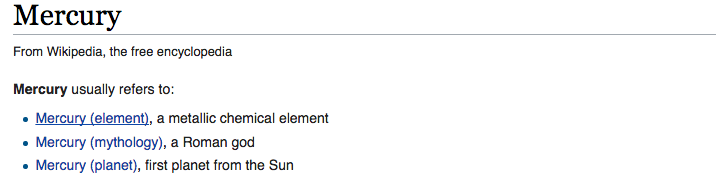
\includegraphics[width=\linewidth]{desambiguation}
  \caption{Disambiguation page for the term ``Mercury".}
  \label{fig:mercury-desambiguation}
\end{figure}


Another variant of Wikilinks is the redirect, employed when different textual forms refer to a single concept or entity. This situation would cause a conflict with the restriction of the uniqueness of titles, imposing the repetition of the content but with different titles. 

The redirect pages contain only text in the form of a directive without gender, number, or case. The central purpose is to find a single article for equivalent terms. For example, if the user searches for ``apples" (plural) the redirect page will refer them to the ``apple" (singular) article. 

Redirections also occur with people's names, when they are known both by their full name and by part of their name or surname. It is the case of the English writer  J. R. R. Tolkien, well-known only by his last name, Tolkien.

\subsubsection{\hspace*{3pt} Infoboxes}

According to Wikipedia documentation\footnote{https://en.wikipedia.org/wiki/Help:Infobox}, infoboxes are fixed-format tables that summarize relevant aspects of an article. It is an optional feature, but they present common attributes between different subjects. Wikipedia recommends the use of a predefined infobox template, as they already have known suggested attributes. 

When editors use predefined infoboxes in an article, Wikipedia displays the table with special formatting that enriches the visual aspect of the box. They are also used as metadata by projects such as DBpedia. Figure \ref{fig:mercury-infobox} shows the infobox for the article on Mercury (a god in Roman religion and mythology).%, displaying the template ``Infobox deity". 



\begin{figure}[!h]
\centering
  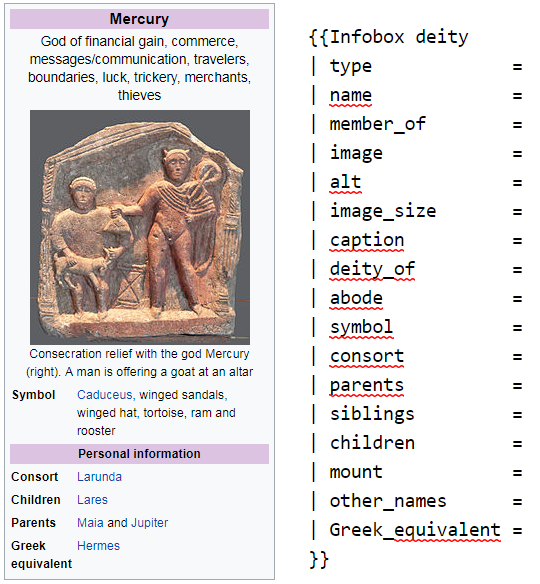
\includegraphics[width=0.8\linewidth]{mercury-infobox}
  \caption{Example Infobox of the page related to the god Mercury with the default properties for infoboxes about deities.}
  \label{fig:mercury-infobox}
\end{figure}



\subsubsection{\hspace*{3pt} Categories}

Every Wikipedia article should have at least one category. Categories are collections that identify topics in the encyclopedia. It should be noted that although the structure of the Wikipedia categories form a taxonomy, it is not represented by a simple tree of subcategories but, in fact, by a complex graph. This graph allows multiple simultaneous categorizations of topics, which means that one category may have multiple parents. The category "Semantics" is a good example of this complex structure since it is a subcategory of ``Grammar",  ``Linguistics", ``Concepts in logic", ``Semiotics", ``Philosophy of language" and others as demonstrated in figure \ref{fig:semantics-category}.


\begin{figure}[H]
\centering
  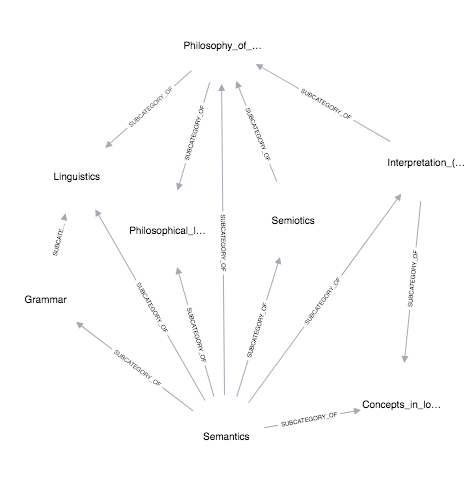
\includegraphics[width=0.8\linewidth]{graph-semantics}
  \caption{Example of an induced graph showing the supercategories of ``Semantics" in the Wikipedia Category Graph.}
  \label{fig:semantics-category}
\end{figure}

Although not based on semantics, Wikipedia has a set of characteristics, such as the definition of a large number of articles and organization of articles in categories, which make it an essential semantic resource. A simple example, but one that illustrates the complexity of the relationships between Wikipedia categories well, is the ``Apple" concept (the fruit), which is directly linked to four categories: ``Apples", ``Malus", ``Fruits originating in Asia", and ``Plants described in 1768". Each of these categories has been added and curated by people who are part of the Wikipedia community. In addition to the explicit knowledge in the directly attributed categories, a vast quantity of implicit knowledge can be inferred by the relations between them, both generically and specifically. Taking the category ``Apples'' as the starting point, links can be followed to the top of the classification system, in what can be perceived as a more generic case: Apples $\rightarrow$  Edible Fruits $\rightarrow$ Edible Plants $\rightarrow$ Food $\rightarrow$ Food and Drink $\rightarrow$ Health.
A more specific case can be illustrated by taking the ``Malus'' category as the origin, and analyzing one of the possible paths to the top: Malus $\rightarrow$ Maleae $\rightarrow$ Prunoideae $\rightarrow$ Rosaceae $\rightarrow$ Rosales $\rightarrow$ Rosids $\rightarrow$ Core Eudicots $\rightarrow$ Eudicots $\rightarrow$ Angiosperms $\rightarrow$ Plants $\rightarrow$ Eukaryota $\rightarrow$ Organisms $\rightarrow$ Life.
These are examples capture small fragments in Wikipedia's categorization structure for the ``Apple" concept. The complete structure involves 33 different categories and 42 different relations between them (See figure \ref{fig:semantics-category-apple}).


\begin{figure}[H]
\centering
  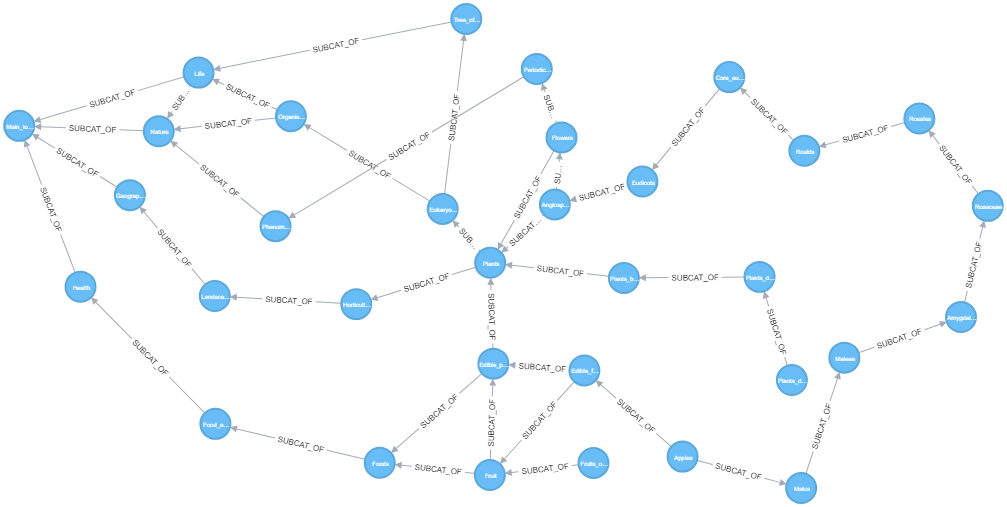
\includegraphics[width=0.8\linewidth]{graph}
  \caption{Example of an induced graph showing the categories and relationships for the Entity Apple towards Main topics}
  \label{fig:semantics-category-apple}
\end{figure}


%\subsection{\hspace*{3pt} DBpedia}

%As described directly on the DBpedia about page\footnote{url{https://wiki.dbpedia.org/about}} DBpedia is a crowd-sourced community effort to extract structured content from the information created in various Wikimedia projects. This structured information resembles an open knowledge graph (OKG) which is available for everyone on the Web. A knowledge graph is a particular kind of database which stores knowledge in a machine-readable form and provides a means for information to be collected, organized, shared, searched and utilized.

%The DBpedia dataset has many advantages compared to the raw data from Wikipedia. Besides the more convenient access to the underlying Wikipedia data sources, it also provides a higher data quality. The higher quality is because the extraction framework embeds multiple steps commonly found in data mining applications, such as duplicate removal in the form of mapping redundant infobox properties to the same DBpedia property.
%Therefore, the present work is focussed on using DBpedia for the entity named recognition and Linking, as well as for traversing entities' categories.

%\subsubsection{\hspace*{3pt} SPARQL}

%\gls{sparql} is a query language capable of retrieving and manipulating data stored in the \gls{rdf} format that is the basis of the OWL language. \gls{rdf} is a labeled and directed data format used to represent information on the Web \cite{prud2008sparql}. 

%In the context of this research, our approach exploits a small part of what the SPARQL language can provide. We navigate in the DBpedia hierarchy to retrieve broader semantic relations between the entities and its categories. 


\subsection{\hspace*{3pt} The Wikipedia Category Graph (WCG)}

Regarding the reduction of dimensionality, a proposed method consists of navigating the \gls{wcg} from each category extracted related to the entities obtained from the text-based resources towards the top of the graph, by all the shortest paths between the category and a set of top-level categories. 

The \gls{wcg} mentioned above is a set of almost 1,500 categories, describing a broad domain of knowledge and ranging from the very precise, such as ``Lists of Canadian network television schedules”, to the very general, such as ``information”. The categories are connected by hypernym relationships, with a child category having an ``subcategory-of” relationship to its parents in the direction of the relationship. However, the graph is not strictly hierarchic: shortcuts exist in the connections (i.e., starting from one child category and going up two different paths of different lengths to reach the same parent category) as well as loops (i.e., beginning from one child category and going up a path to reach the same child category again).

Given the complexity and dimension of the \gls{wcg}, a graph-theoretic analysis was carried out and is described in Chapter \ref{chapter:graph}. 
